\chapter{Production d'une source cohérente d'ondes de matière}
\label{ch:BECmanip}
%\begin{tikzpicture}[remember picture, overlay]
%\node[anchor=north east,inner sep=0pt] at (current page.north east) {
\includegraphics[scale=1]{Fig/Chapter1/g825.png}};
%\end{tikzpicture}


interaction lumière-atome, BEC, principales étapes de refroidissement. 

\section{Condensation de Bose-Einstein}
\subsection{Statistique de Bose-Einstein}
%\subsection{Équation de Gross-Pitaevskii}
\subsection{Propriétés d'un condensat de Bose-Einstein}

\section{Processus d'interaction lumière-matière} 
\subsection{Potentiel dipolaire}
\subsection{Force de pression de radiation}
\subsection{Potentiel magnétique}
\subsection{Couplage radio-fréquence} 

\section{Description d'un cycle expérimental}
\subsection{Première chambre}
\subsection{Chambre de science}
\subsection{Imagerie}




\begin{comment}
%Chapter 3: A cognitive experiment to study confidence
%------------------------

%3.1 : Experimental procedure
%- In humans
%- In animals


%3.2 : Our procedure


%% Intro à retravailler

Confidence judgments in one's decision are considered a central example of metacognition. How can we access to the subjective sense of confidence of someone else ? In this chapter, I will review to different behavioral measures to obtain this sense of confidence in humans and in animals. In a second part, I will present the experiment I performed, in collaboration with Jean-R\'emy Martin and J\'er\^ome Sackur at ENS, during my PhD. 


\section{How to measure confidence experimentally ?}

%% plus  de refs si le temps

%% exemple des histogrammes et des performances etc ....
%% une partie sur les inconvenients d'une telle méthode
% https://link.springer.com/article/10.3758/s13423-018-1553-3

\subsection{In Humans} %% titre à changer

\paragraph*{Explicit reports of confidence}
Reports of confidence in humans can be made explicit through verbal communications for example.Thus, the most straightforward paradigm to measure confidence is to ask the subjects to assign a numerical rating in how sure they are in their answer at each trial. %% REFS
They provide a subjective probability on the correctness of their response as a confidence judgment.
One important aspect of such reports is that performance accuracy and response times are well-correlated with self-confidence reports. %ù REFS
This phenomena occurs for a variety of tasks such as general knowledge tests~\citep{perfect1993accuracy}, perceptual decisions~\citep{fleming2010relating} and reasoning tasks~\citep{stankov2000complexity}.
%% Figure suivante faite grâce à la base de donnée confidence database Adler & ma 2018 exp 2
In Figure ???, I represent an example of such relation between these behavioral variables. The experiment consisted in a categorization task (with Gabor patches) followed by a confidence judgment on a four-points scale. %% REF Adlmer
The data are publicly shared through the {\em confidence databse} project. %% REFS
The most striking effect that appears from having access to direct reports of confidence is the {\em under/over-confidence}~\citep{lichtenstein1977those}. %% A lire plus en détails TODO TODO TODO ++++
These deviations occur systematically with overconfidence when the decisions are difficult and underconfidence for easy decisions~\citep{Kepecs_A_2012}. 
However, it is worth noting that these biases in confidence vary greatly with the type of judgments that are asked, and across participants~\citep{klayman1999overconfidence}. %% Figure overconfidence à faire en exemple

%% remarque sur version cntinue, discrète ou combien d'échelon



%% un mot sur les autres méthodes
\paragraph*{Other measures of confidence}

%\paragraph*{Post-decision wagering} for exemple

%% lire les autres articles pour bien comprendre les critiques/remarques
%% lesm oyens de mesures sont très variés (article Pascal M.)

%% formulatio à revoir
\subsection{In animals}
For animals, one can not simply ask them to explicitly report their confidence. Therefore, more sophisticated tasks have been employed to elicit a report of confidence in animals.

\paragraph*{Uncertain option task} %%%REFS ??? et article shadlen ?
One of the most common task used for this purpose is the {\em uncertain option} task. It extends the classical two-choices paradigm that has been mentioned in this thesis. In addition to the two available responses, the animal is offered a third choice, that will correspond to a small but certain reward. This framework has been used in many species such as monkeys, dolphin and rats. %% REFS 
Interestingly, when compared to human performances on this type of task, dolphin and monkeys showed qualitative similar strategies and response distributions. However, one can address the following criticism to this kind of task: there is the possibility that this task is considered as a three-choices task by the animal. The animal could be learning the association between the uncertain reward and a difficult task. 


\paragraph*{Opt-out task}
% expliquer marche pas avec rat (sauf exception) et donc les exp. suivantes
% fig inkscape opt-out task
To address this problematic,~\cite{hampton2001rhesus} developed a modified version of the uncertain option task. It consists in a memory task in which monkeys perform a delayed-maching-to-sample task. At the end of delay, monkeys were presented with the option of declining or accepting the discrimination test. Moreover,~\cite{hampton2001rhesus} imposed that on some trials the monkeys have no choice but to make the discrimination test. This is to ensure that the monkey is not learning to associate longer delay with {\em opt-out option}. They found that, the performances of the monkeys on freely chosen trials are greater than the ones in forced choice trials. 
This opt-out task as been used in macaque monkeys too~\citep{kiani2009representation,komura2013responses}, but in binary categorization of visual motion task. They found that the frequency of choosing the opt-out option increased with stimulus difficulty, as well as greater performances on freely chosen trials. Interestingly, this task has been tested in pigeons and rats %% REFS
but they don't find a change in performances between forced-choices and free-choices. These results raised the question or whether these animals could perform confidence judgments or not.



\paragraph*{Decision restart and leaving decision tasks}
%% un mot sur les problematiques de cette tache ?


In order to address the criticisms of two previous paradigms, such as the fact that, for these paradigms, either a confidence report either a decision report is collected at each trial,~\cite{Kepecs_A_2012} proposed a new paradigm in rodents. %% Figure %ù TODO phrase un peu longue ???
The rats were trained to perform a 2AFC olfactory discrimination task. Depending on the dominant part of the odour mixture, the rats need to choice the left or the right. A variable delay was imposed after a correct trial and the animal could restart the trial at will (Figure ???). There was no feedback on error trials which allow to measure the rats confidence in these trials. For some of the correct trials, the reward was omitted which allow to measure confidence for correct trials too. It has been found that the waiting time increased with respect to odour contrast for correct trials, but decreased for error trials. Moreover, accuracy was an increasing function of the waiting time. This suggests that the waiting time of each trial consists in a robust proxy for confidence.


\begin{figure}[h!]
	\centering
	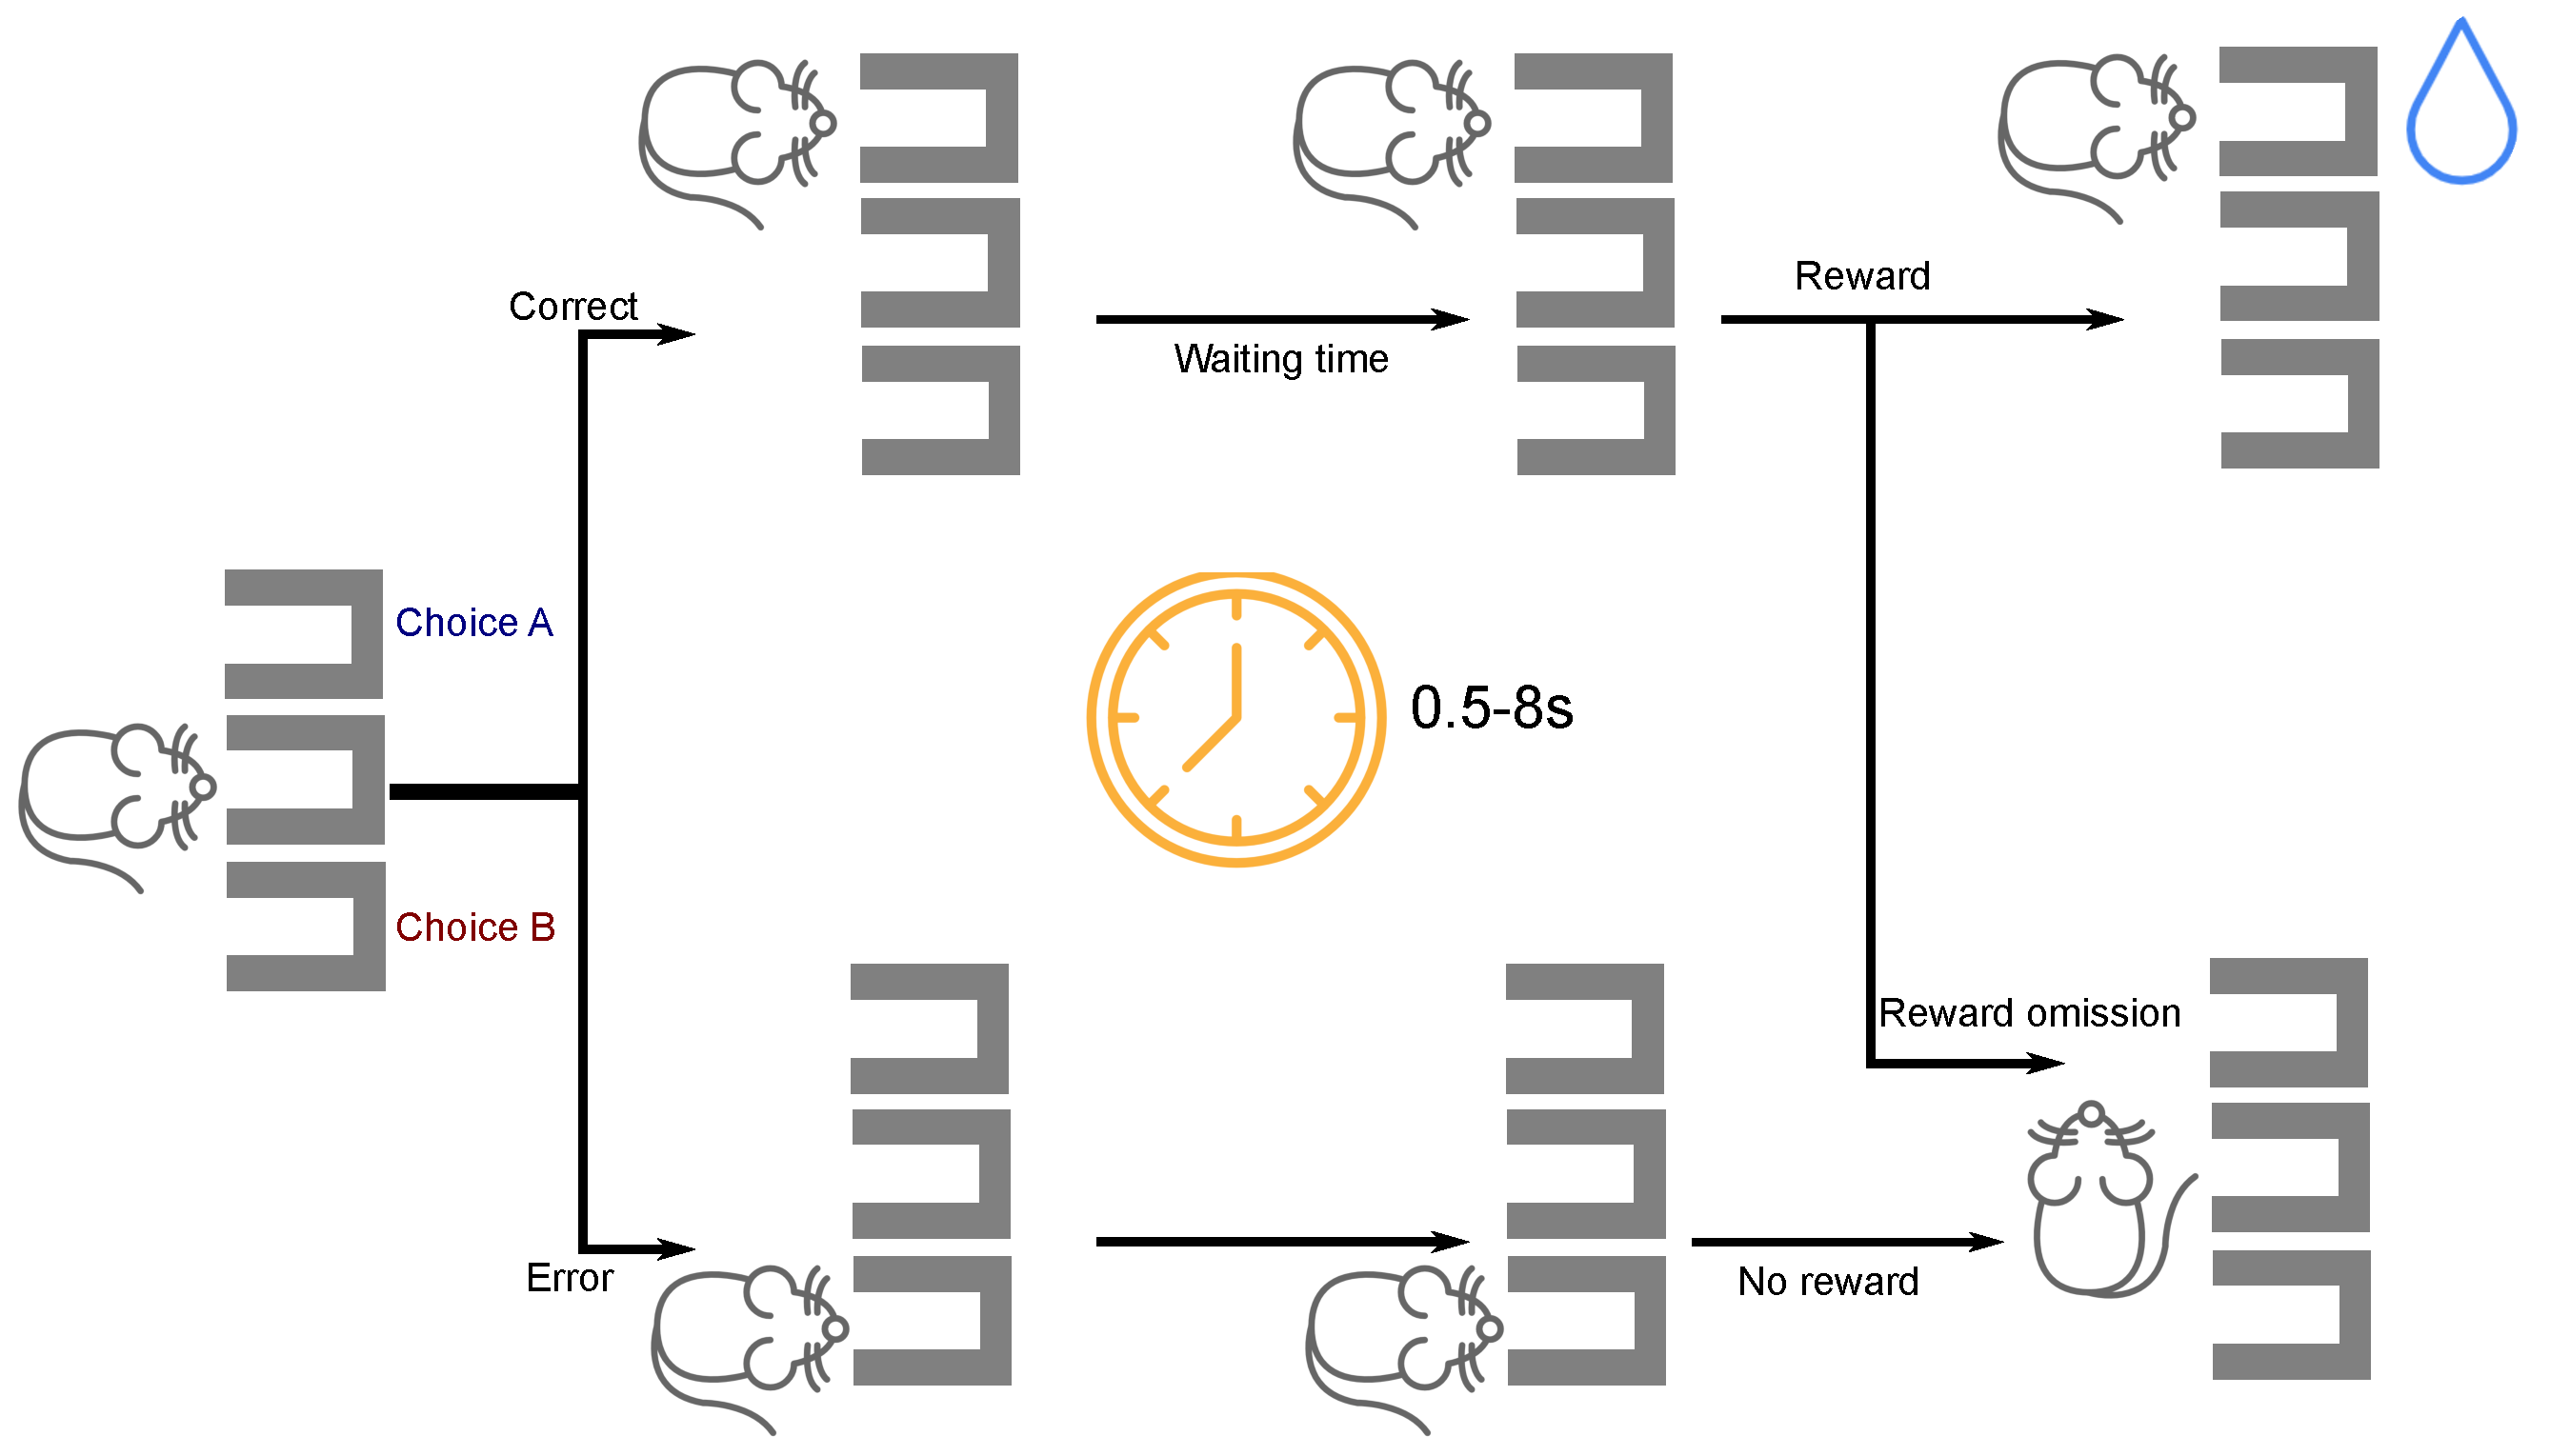
\includegraphics[width=0.7\linewidth]{Fig/Chapter3/confidence-souris.eps}
	\caption{{\bf }
	}
	\label{fig:fig6}
\end{figure}

%% conclusion de la section ????


\section{My experiment}

In this section I will describe the cognitive experiment that I have performed to study decision-making and confidence in humans. Previously to the design of this experiment, I briefly analyzed the results of an experiment of Jean-R\'emy Martin and J\'er\^ome Saclur within the framework of attractor neural network. The preliminary results led to the design of an experiment whose goal was to study the impact of confidence on decision-making and various sequential effects.


\subsection{Experimental set-up}
The experiment was performed at the Laboratoire de Psychologie cognitive et de Psycholinguistique’s database (LSCP, DEC, ENS-EHESS-CNRS, PSL, Paris, France). The experiment followed the ethics requirements of the Declaration of Helsinki (2008) and has been approved by the local Ethics Committee. It consists in a direction categorization task, where participants classify Gabor patches as clockwise or anti-clockwise. In some of the trials, the decision was followed by an auditory feedback or a confidence evaluation.

%% photo des salles de manip
The stimuli were generated using Matlab along with the Psychophysics toolbox. %% PERFS
The ywere displayed on a monitor at $57.3$~cm of the particpants head. The participants performed the experiment
in a quiet and darkened experimental room. Their heads were stabilized thanks to a chin-rest. %% Figure ????
The instructions to the participants (translated from french) were the following (the emphazised sentences correspond to additional information not provided to the participants):
\begin{itemize}
	\item In each trial, you will see very briefly ({\em $200$~ms}) a black dot at the center of the screen that you will need to look at (Figure~\ref{fig:consignes1}.A). Just after the dot dissappears ({\em ???~ms}), you will see a circular grating at the center of the screen like the one in Figure~\ref{fig:consignes1}.B. {\em The parameters of the circular grating are diameter = $4^{\circ}$, Tukey window, 2 cycles per degree, Michelson contrast = $89\%$, duration = $100$~ms, phase randomly selected at each trial.}
	
	\begin{figure}[h!]
		\begin{subfigure}{.5\textwidth}
			\centering
			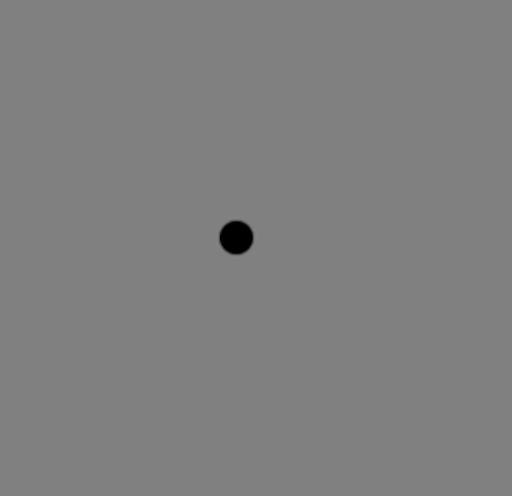
\includegraphics[width=.8\linewidth]{fig/Chapter3/fixation-dot.png}
			\caption{Fixation dot}
		\end{subfigure}%
		\begin{subfigure}{.5\textwidth}
			\centering
			
\includegraphics[width=.8\linewidth]{fig/Chapter3/0-grating.png}
			\caption{Example of the circular grating.}
		\end{subfigure}
		\caption{}
		\label{fig:consignes1}
	\end{figure}
	
	
	
	\item In each trial you will need to indicate if the grating was oriented clockwise or anti-clockwise (Figure~\ref{fig:consignes2}).
	\item As soon as the disk dissappears, if you think it was anti-clockwise oriented you will press the left directionnal arrow. If it was clockwise oriented you will press the right directionnal arrow.
	
		\begin{figure}[h!]
		\begin{subfigure}{.5\textwidth}
			\centering
			
\includegraphics[width=.8\linewidth]{fig/Chapter3/left-grating.png}
			\caption{Anti-clockwise circular grating.}
		\end{subfigure}%
		\begin{subfigure}{.5\textwidth}
			\centering
			
\includegraphics[width=.8\linewidth]{fig/Chapter3/right-grating.png}
			\caption{Clockwise circular grating.}
		\end{subfigure}
		\caption{}
		\label{fig:consignes2}
	\end{figure}
	
	
	\item In the case where you don't know at all which direction it was you will still press one of the two keys by following your intuition. When this happens, do not press always the same key.
	\item You need to answer fast but not at the expense of accuracy. After $1.5$ second, you will see a message at the screen "Please, answer". The ideal situation is to answer before this text appears at the screen.
	\item You will have $3$ bocks of trials:
	\begin{itemize}
		\item In the first block, once you have answered to a trial, the software will automatically run the next trial.
		\item  In a second block, you will receive a feedback on your answer at each trial. If the answer was correct, you will hear a pitched tone. If your answer was wrong you will hear a deep tone.
		\item In a third block, you will need to evaluate your confidence level in your answer using the scale that will appear on the screen (Figure ??). You will move the black slider towards right or left using the left and right stickers on the keyboard (q and e keys). The scale is composed of $10$ levels. The case at the left corresponds to the "Pure guessing" case. You choose randomly the orientation of the grating. At the right you have the "Certain to be sure" case. You are absolutely certain to be right, there is no possible doubt. Between these two cases, you have access to intermediate levels of confidence. The choice of the confidence level is performed using the space bar.
			
			
				\begin{figure}[h!]
					\centering
					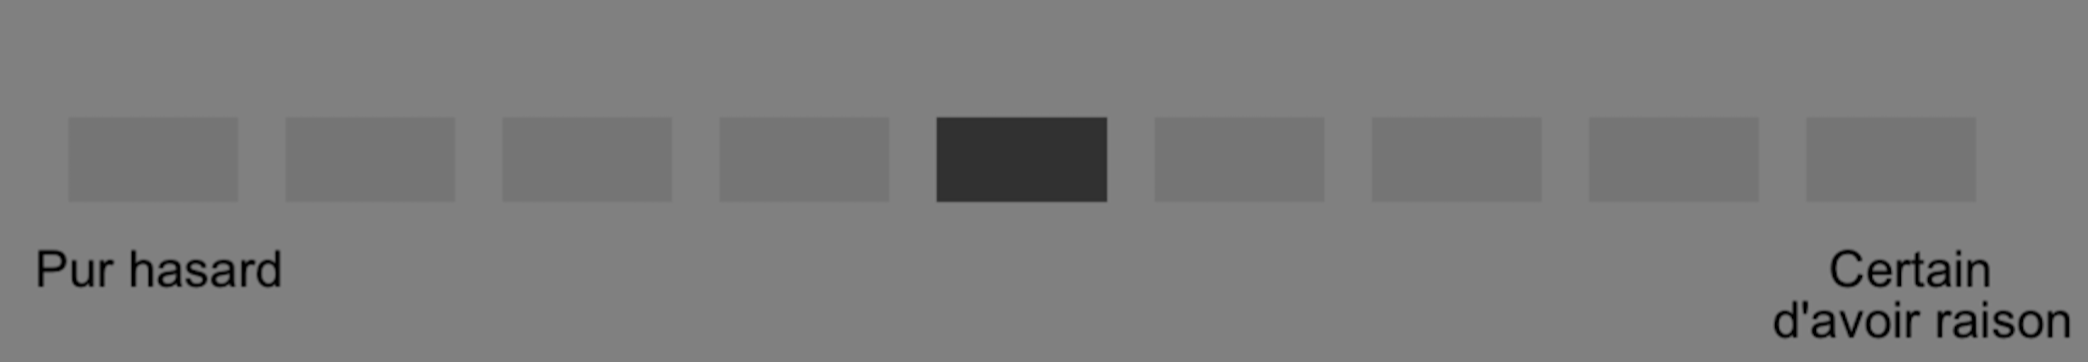
\includegraphics[width=.8\linewidth]{fig/Chapter3/scale-confidence.png}
					\caption{Confidence-scale.}
					\label{fig:consignes3}
			\end{figure}
			
			
			
	\end{itemize}
\item Be aware that, in the confidence block, the black slider will appear randomly on the scale. Don't be biased by the initial position of the cursor and move it o the level that reflets your level of confidence.
\item During the confidence block, in the case you wanted to choose the right arrows but you chose the left one (or inversely), don't answer to the confidence scale. Just press the keyboard key with a red sticker on it, it will go to the next trial.
\item The software will choose the order of the block and you will know at the beginning of each block which one it is. Before the main experiment starts, you will have a small training.
\end{itemize}

Nine participants (7 Females, Mean Age = 27.3, SD = 5.14) have been recruited from the Laboratoire de Psychologie cognitive et de Psycholinguistique’s database (LSCP, DEC, ENS-EHESS-CNRS, PSL, Paris, France).
Every subject had normal or corrected-to-normal vision. The participants performed three sessions on three distinct days in the same week for a total duration of about 2h15. Three participants were excluded. Two of the excluded participants did not complete correctly the experiment and one exhibited substantially asymmetric performance
($98\%$ of correct responses for an angle of 0.2\textdegree, but $18\%$ at -0.2\textdegree degree). As a result, we analyzed data from 6 participants. We obtained written informed consent from every participant who received a compensation of 15 euros for their participation. 
Participants performed three sessions on three distinct days. Each session ($45$~min) consisted in three runs, each run being composed of one exemplar of each of the three type of block, in a random order.




\subsection{Experimental procedure}

The experimental procedure is shown in Figure ??. The waiting time between each trial was deliberatly chosen to be low, and similar between blocks, to study the sequential effects.



\paragraph*{Pure block} 
In this block, participants waited $300$~ms after each decision, before the black fixation point appears. The stimulus appeared $200$~ms after this fixation point. The eight possible orientations for the circular grating were [-1.6\textdegree, -0.8\textdegree, -0.5\textdegree, -0.2\textdegree , 0.2\textdegree , 0.5\textdegree , 0.8\textdegree , 1.6\textdegree  ] and a stimulus was chosen randomly among them with the following weights: [0.05, 0.1, 0.15, 0.2, 0.2, 0.15, 0.1, 0.05]. 

\paragraph*{Feedback block}
In this block, $200$~ms after the decision, the participants received an auditory feedback (during $200$~ms) about the correctness of the decision they just made. The black fixation dot appeared $100$~ms after this feedback and a new trial began. The orientations of the circular gratings were chosen randomly from [-1.6\textdegree, -0.8\textdegree,  -0.2\textdegree , 0.2\textdegree ,  0.8\textdegree , 1.6\textdegree  ] with the following weights [ 0.12, 0.18, 0.2, 0.2, 0.18, 0.12 ].


\paragraph*{Confidence block} In the confidence block, participants had to evaluate the confidence on the orientation task $200$~ms after the decision. After the choice of confidence, the participants had to wait $300$~ms before the black fixation dot appears. After the fixation dot the stimulus appeared $200$~ms later. The orientations of the circular gratings were the same as in the feedback block. 

%%% différents résultats des performances etc ....
%% testi nfluence block confiance

I will present different results from this experiment, without the framework of attractor network that will be discussed in the next chapter of this manuscript. 



\end{comment}


